\section{Improper Integrals}\label{sec:ImproperIntegrals}
%%%%%%%%%%%%%%%%%%%%%%%%%%%%%%%%%%%%%%%%%%%%%%%%%%%
Recall that the Fundamental Theorem of Calculus says that if $f$ is a \underline{{\bf continuous}} function on the closed interval $[a,b]$, then
$$\ds{\int_a^b f(x)~dx=F(x)\bigg|_a^b=F(b)-F(a)},$$
where $F$ is any antiderivative of $f$. 

Both the {\bf continuity} condition and {\bf closed interval} must hold to use the Fundamental Theorem of Calculus, and in this case, $\ds\int_a^b f(x)\,dx$ represents the net area under $f(x)$ from $a$ to $b$: 
$$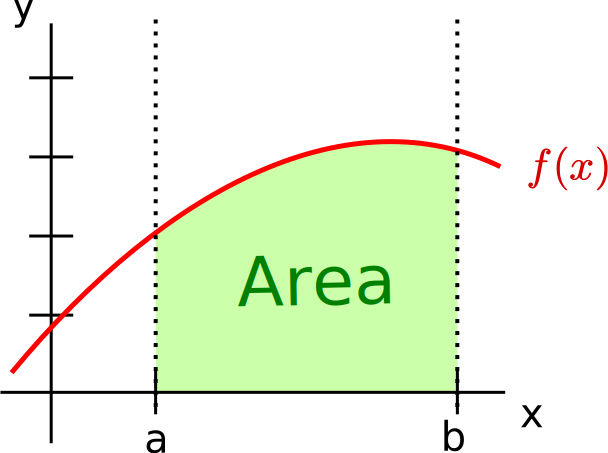
\includegraphics[width=2.25in]{images2/area-under}$$

We begin with an example where blindly applying the Fundamental Theorem of Calculus can give an incorrect result.

\begin{example}{Using FTC}{Using FTC}
Explain why $\ds\int_{-1}^1\frac{1}{x^2}\,dx$ is not equal to $-2$.
\end{example}  

\begin{solution}
Here is how one might proceed:  
$$
\int_{-1}^1\frac{1}{x^2}\,dx 
~=~ \int_{-1}^1 x^{-2}\,dx 
~=~ -x^{-1}\bigg|_{-1}^1 
~=~ -\frac{1}{x}\bigg|_{-1}^1 
~=~ \left(-\frac{1}{1}\right) - \left(-\frac{1}{(-1)}\right) 
~=~ -2$$  
 However, the above answer is {\bf WRONG!} 
 Since $f(x)=1/x^2$ is not continuous on $[-1,~1]$, we cannot directly apply the Fundamental Theorem of Calculus.
Intuitively, we can see why $-2$ is not the correct answer by looking at the graph of $f(x)=1/x^2$ on $[-1,~1]$.
The shaded area appears to grow without bound as seen in the figure below.
$$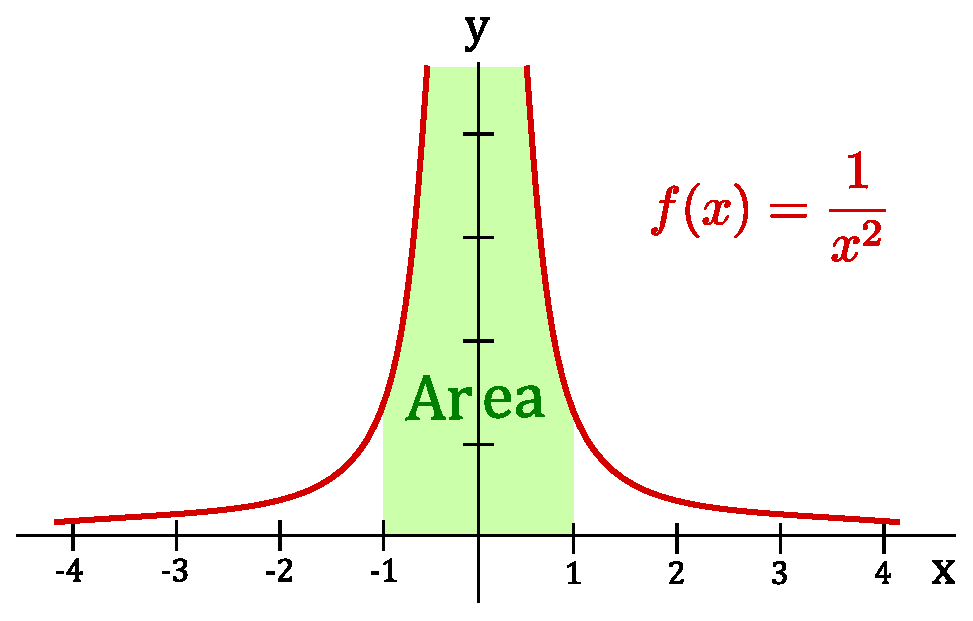
\includegraphics[width=2.5in]{images2/improper-integral-example-1}$$
\end{solution}

Formalizing this example leads to the concept of an improper integral.
There are two ways to extend the Fundamental Theorem of Calculus.
One is to use an {\bf infinite interval}, i.e., $[a,\infty)$, $(-\infty,b]$ or $(-\infty,\infty)$.
The second is to allow the interval $[a,b]$ to contain an infinite {\bf discontinuity} of $f(x)$.
In either case, the integral is called an {\bf improper integral}.  
One of the most important applications of this concept is probability distributions.  

To compute improper integrals, we use the concept of limits along with the Fundamental Theorem of Calculus.
 
\begin{definition}{Definitions for Improper Integrals}{Definitions for Improper Integrals}
If $f(x)$ is continuous on $[a,\infty)$, then the improper integral of $f$ over $[a,\infty)$ is:
$$\int_{a}^{\infty} f(x)\,dx:=\lim_{R\to\infty}\int_a^R f(x)\,dx.$$ 
If $f(x)$ is continuous on $(-\infty,b]$, then the improper integral of $f$ over $(-\infty,b]$ is:
$$\int_{-\infty}^b f(x)\,dx:=\lim_{R\to -\infty}\int_R^b f(x)\,dx.$$
\end{definition}

If the limit exists and is a finite number, we say the improper integral {\bf converges}. Otherwise, we say the  improper integral {\bf diverges}.

To get an intuitive (though not completely correct) interpretation of improper integrals, we attempt to analyze $\ds\int_a^\infty f(x)\,dx$ graphically. 
 Here assume $f(x)$ is continuous on $[a,\infty)$: 
$$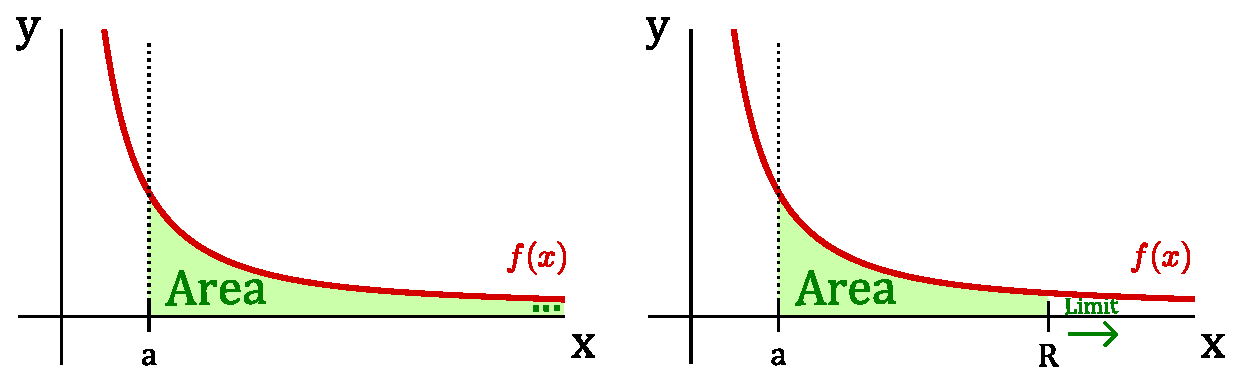
\includegraphics[width=5in]{images2/improper-integral-theory-2}$$ 
 We let $R$ be a fixed number in $[a,\infty)$. 
 Then by taking the limit as $R$ approaches $\infty$, we get the improper integral:  
$$\int_a^\infty f(x)\,dx:=\lim_{R\to\infty}\int_a^R f(x)\,dx.$$ 
 We can then apply the Fundamental Theorem of Calculus to the last integral as $f(x)$ is continuous on the closed interval $[a,R]$.

We next define the improper integral for the interval $(-\infty,~\infty)$.

\begin{definition}{Definitions for Improper Integrals}{Definitions for Improper Integrals}
 If both $\ds\int_{-\infty}^a f(x)\,dx$ and $\ds\int_{a}^{\infty} f(x)\,dx$ are convergent, then the improper integral of $f$ over $(-\infty,\infty)$ is:
$$\int_{-\infty}^{\infty} f(x)\,dx:=\int_{-\infty}^a f(x)\,dx+\int_{a}^{\infty} f(x)\,dx$$
\end{definition}

The above definition requires {\bf both} of the integrals
$$\int_{-\infty}^a f(x)\,dx\qquad\mbox{and}\qquad\int_{a}^{\infty} f(x)\,dx$$
to be convergent for $\ds\int_{-\infty}^{\infty} f(x)\,dx$ to also be convergent. 
 If {\bf either} of $\ds\int_{-\infty}^a f(x)\,dx$ or $\ds\int_{a}^{\infty} f(x)\,dx$ is divergent, then so is $\ds\int_{-\infty}^{\infty} f(x)\,dx$.

\begin{example}{Improper Integral}{Improper Integral}
Determine whether $\ds\int_1^\infty\frac{1}{x}\,dx$ is convergent or divergent.
\end{example} 

\begin{solution}
 Using the definition for improper integrals we write this as:
$$	\int_1^\infty \frac{1}{x}\,dx= \lim_{R\to\infty} \int_1^R\frac{1}{x}\,dx
	= \lim_{R\to\infty} \ln|x|\bigg|_1^R
	=\lim_{R\to\infty} \ln|R| - \ln|1|
	= \lim_{R\to\infty} \ln|R|
	= +\infty$$
 Therefore, the integral is {\bf divergent}.
\end{solution}

\begin{example}{Improper Integral}{Improper Integral}
Determine whether $\ds\int_{-\infty}^\infty x\sin(x^2)\,dx$ is convergent or divergent.
\end{example}  

\begin{solution}
 We must compute both $\ds\int_0^\infty x\sin(x^2)\,dx$ and $\ds\int_{-\infty}^0 x\sin(x^2)\,dx$.  
 Note that we don't have to split the integral up at $0$, any finite value $a$ will work.  
 First we compute the indefinite integral.  
 Let $u=x^2$, then $du=2x\,dx$ and hence, 
$$\int x\sin(x^2)\,dx=\frac{1}{2} \int \sin(u)\,du=-\frac{1}{2}\cos(x^2)+C$$
Using the definition of improper integral gives: 
$$\int_0^\infty x\sin(x^2)\,dx  =  \lim_{R\to\infty} \int_0^R x\sin(x^2)\,dx 
=\lim_{R\to\infty} \left[-\frac{1}{2}\cos(x^2)\right] \bigg|_0^R 
=  -\frac{1}{2} \lim_{R\to\infty} \cos(R^2) +\frac{1}{2}$$
This limit does not exist since $\cos x$ {\bf oscillates} between $-1$ and $+1$. 
 In particular, $\cos x$ does not approach any particular value as $x$ gets larger and larger. 
 Thus, $\ds\int_0^\infty x\sin(x^2)\,dx$ diverges, and hence, $\ds\int_{-\infty}^\infty x\sin(x^2)\,dx$ diverges.
\end{solution}

When there is a discontinuity in $[a,b]$ or at an endpoint, then the improper integral is as follows.

\begin{definition}{Definitions for Improper Integrals}{Definitions for Improper Integrals}
If $f(x)$ is continuous on $(a,b]$, then the improper integral of $f$ over $(a,b]$ is:  
$$\int_a^b f(x)\,dx:=\lim_{R\to a^+}\int_R^b f(x)\,dx.$$  
If $f(x)$ is continuous on $[a,b)$, then the improper integral of $f$ over $[a,b)$ is:  
$$\int_a^b f(x)\,dx:=\lim_{R\to b^-}\int_a^R f(x)\,dx.$$
\end{definition}

If the limit above exists and is a finite number, we say the improper integral {\bf converges}.
Otherwise, we say the improper integral {\bf diverges}. 

When there is a discontinuity in the interior of $[a,b]$, we use the following definition.

\begin{definition}{Definitions for Improper Integrals}{Definitions for Improper Integrals}
If $f$ has a discontinuity at $x=c$ where $c\in[a,b]$, and both
both $\ds\int_a^c f(x)\,dx$ and $\ds\int_c^b f(x)\,dx$ are convergent, then $f$ over $[a,b]$ is:  
$$\int_a^b f(x)\,dx:=\int_a^c f(x)\,dx+\int_c^b f(x)\,dx$$
\end{definition}

Again, we can get an intuitive sense of this concept by analyzing $\ds\int_a^b f(x)\,dx$ graphically. 
Here assume $f(x)$ is continuous on $(a,b]$ but discontinuous at $x=a$: 
$$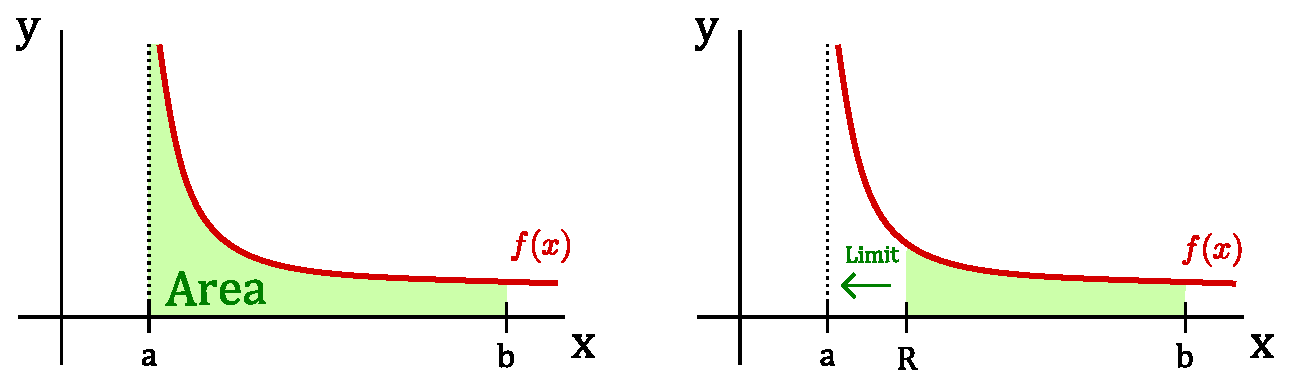
\includegraphics[width=5in]{images2/improper-integral-theory-1}$$ 
 We let $R$ be a fixed number in $(a,b)$. 
 Then by taking the limit as $R$ approaches $a$ from the {\bf right},  we get the improper integral: 
$$\int_a^b f(x)\,dx:=\lim_{R\to a^+}\int_R^b f(x)\,dx.$$ 
 Now we can apply FTC to the last integral as $f(x)$ is continuous on $[R,b]$.

\begin{example}{A Divergent Integral}{A Divergent Integral}
Determine if $\ds\int_{-1}^1\frac{1}{x^2}\,dx$ is convergent or divergent.
\end{example}  

\begin{solution}
 The function $f(x)=1/x^2$ has a discontinuity at $x=0$, which lies in $[-1,1]$.  
 We must compute $\ds\int_{-1}^0 \frac{1}{x^2}\,dx$ and $\ds\int_0^1 \frac{1}{x^2}\,dx$. Let's start with $\ds\int_0^1 \frac{1}{x^2}\,dx$:  
$$\int_0^1 \frac{1}{x^2}\,dx = \lim_{R\to 0^+} \int_R^1 \frac{1}{x^2} \,dx = \lim_{R\to 0^+} -\frac{1}{x}\bigg|_R^1
= -1 + \lim_{R\to 0^+} \frac{1}{R}$$
which diverges to $+\infty$.
 Therefore, $\ds\int_{-1}^1\frac{1}{x^2}\,dx$ is {\bf divergent} since one of $\ds\int_{-1}^0 \frac{1}{x^2}\,dx$ and $\ds\int_0^1 \frac{1}{x^2}\,dx$ is divergent.
\end{solution}


% % % % % % %
% % The following example 'Integral of the Logarithm' can be replaced with the next example if Integration by Parts is not included in the text adaptation.
\begin{example}{Integral of the Logarithm}{Integral of the Logarithm}
Determine if $\ds\int_0^1 \ln x \,dx$ is convergent or divergent. Evaluate it if it is convergent.
\end{example}  

\begin{solution}
Note that $f(x)=\ln x$ is discontinuous at the endpoint $x=0$. 
We first use integration by parts to compute $\ds\int\ln x\,dx$.
We let $u=\ln x$ and $dv=dx$.
Then $du=(1/x)dx$, $v=x$, giving:
\begin{eqnarray*}
\int \ln x\,dx &=& \ds x\ln x-\int x\cdot\frac{1}{x}\,dx\\
&=& x\ln x-\int 1\,dx\\
&=& x\ln x-x+C\\
\end{eqnarray*}
 Now using the definition of improper integral for $\ds\int_0^1 \ln x \,dx$: 
$$
	\int_0^1 \ln x \,dx = \lim_{R\to 0^+} \int_R^1 \ln x\,dx 
	=  \lim_{R\to 0^+} (x\ln x-x)\bigg|_R^1 
	%=  \lim_{R\to 0^+} \left(\left[\ln 1-1\right] - \left[R\ln R-R\right]\right)
	=  -1 - \lim_{R\to 0^+}(R\ln R) + \lim_{R\to 0^+}R 
$$
Note that $\ds\lim_{R\to 0^+}R=0$. 
We next compute $\ds\lim_{R\to 0^+}(R\ln R)$.
First, we rewrite the expression as follows:
$$\lim_{x\to0^+}(R\ln R)=\lim_{R\to0^+}\frac{\ln R}{1/R}.$$
Now the limit is of the indeterminate type $(-\infty)/(\infty)$ and l'H\^opital's Rule can be applied.  
$$\lim_{R\to0^+}(R\ln R) =\lim_{R\to0^+}\frac{\ln R}{1/R}
=\lim_{R\to0^+}\frac{1/R}{-1/R^2}
=\lim_{R\to0^+}-\frac{R^2}{R}
=\lim_{R\to0^+}(-R)
=0$$
Thus, $\ds\lim_{R\to 0^+}(R\ln R)=0$.
Thus
$$\int_0^1 \ln x \,dx = -1,$$ 
and the integral is convergent to $-1$. 

Graphically, one might interpret this to mean that the net area under $\ln x$ on $[0,1]$ is $-1$ (the area in this case lies below the $x$-axis). 
$$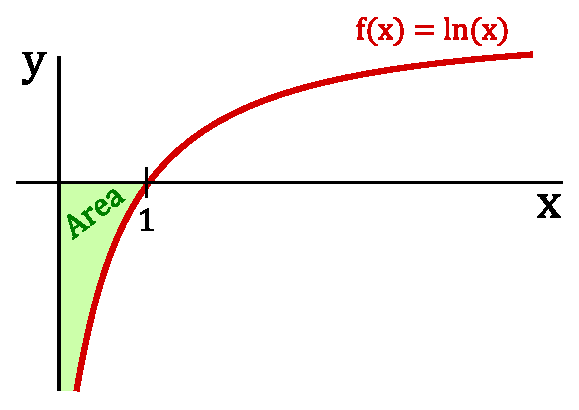
\includegraphics[width=2.5in]{images2/improper-integral-example-2}$$
\end{solution}

\begin{example}{Integral of a Square Root}{IntSquareRoot}
Determine if $\ds\int_0^4\frac{dx}{\sqrt{4-x}}$ is convergent or divergent. Evaluate it if it is convergent.
\end{example}
\begin{solution}
Note that $\frac{1}{\sqrt{4-x}}$ is discontinuous at the endpoint $x=4$. We use a $u$-substitution to compute $\int \frac{dx}{\sqrt{4-x}}$. We let $u=4-x$, then $du=-dx$, giving:
\begin{align*}
\ds\int\frac{dx}{\sqrt{4-x}}&=\int-\frac{du}{u^{1/2}}	\\
&=\int -u^{-1/2}\,du	\\
&=-2(u)^{1/2}+C	\\
&=-2\sqrt{4-x}+C
\end{align*}
Now using the definition of improper integrals for $\ds\int_0^4\frac{dx}{\sqrt{4-x}}$:
\[\ds\int_0^4\frac{dx}{\sqrt{4-x}}=\lim_{R\to4^{-}}(-2\sqrt{4-x})\bigg|_0^R=\lim_{R\to4^{-}}-2\sqrt{4-R}+2\sqrt{4}=4\]
\end{solution}

\begin{example}{Improper Integral}{ImpIntExample}
Determine if $\ds\int_{1}^{2}\dfrac{dx}{\left( x-1\right) ^{1/3}}$ is
convergent or divergent. Evaluate it if it is convergent.
\end{example}
\begin{solution}
Note that $f\left( x\right) =\dfrac{1}{\left( x-1\right) ^{1/3}}$
is discontinuous at the endpoint $x=1.$ We first use substitution to find
$\ds\int \dfrac{dx}{\left( x-1\right) ^{1/3}}.$ We let $u=x-1.$ Then $du=dx,$
giving%
\begin{equation*}
\int \dfrac{dx}{\left( x-1\right) ^{1/3}}=\int \frac{du}{u^{1/3}}=\int
u^{-1/3}du=\frac{3}{2}u^{2/3}+C=\frac{3}{2}\left( x-1\right) ^{2/3}+C.
\end{equation*}%
Now using the definition of improper integral for $\ds\int_{1}^{2}\dfrac{dx}{%
	\left( x-1\right) ^{1/3}}:$%
\begin{equation*}
\int_{1}^{2}\dfrac{dx}{\left( x-1\right) ^{1/3}}=\lim_{R\rightarrow
	1^{+}}\int_{R}^{2}\dfrac{dx}{\left( x-1\right) ^{1/3}}=\left.
\lim_{R\rightarrow 1^{+}}\frac{3}{2}\left( x-1\right) ^{2/3}\right\vert
_{R}^{2}=\frac{3}{2}-\lim_{R\rightarrow 1^{+}}\frac{3}{2}\left( R-1\right)
^{2/3}=\frac{3}{2},
\end{equation*}%
and the integral is convergent to $\frac{3}{2}.$ Graphically, one might
interpret this to mean that the net area under $\dfrac{1}{\left( x-1\right)
	^{1/3}}$ on $\left[ 1,2\right] $ is $\frac{3}{2}$.

$$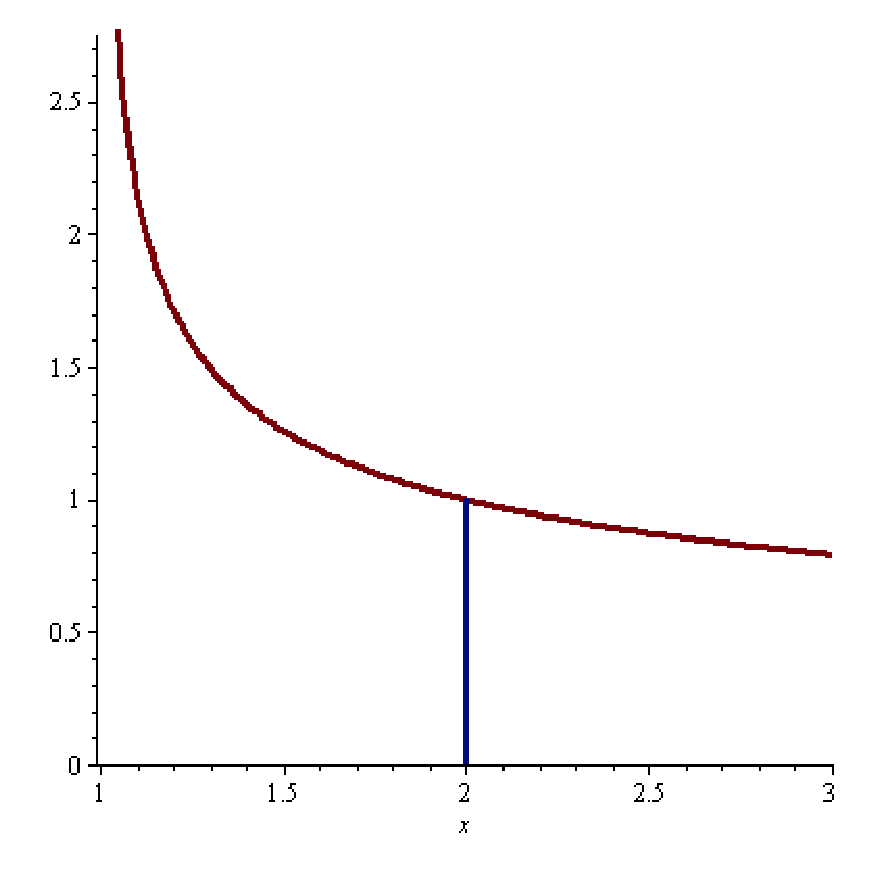
\includegraphics[width=8cm]{images/improper-int-example}$$
\end{solution}

The following test allows us to determine convergence/divergence information about improper integrals that are hard to compute by comparing them to easier ones. 
We state the test for $[a,\infty)$, but similar versions hold for the other improper integrals.

\begin{formulabox}[The Comparison Test]
Assume that $f(x)\geq g(x)\geq 0$ for $x\geq a$.
\begin{enumerate}[(i)]
\item	If $\ds\int_a^\infty f(x)\,dx$ {\bf converges}, then $\ds\int_a^\infty g(x)\,dx$ also {\bf converges}.
\item	If $\ds\int_a^\infty g(x)\,dx$ {\bf diverges}, then $\ds\int_a^\infty f(x)\,dx$ also {\bf diverges}. 
\end{enumerate}
\end{formulabox}

Informally, (i) says that if $f(x)$ is larger than $g(x)$, and the area under $f(x)$ is finite (converges), then the area under $g(x)$ must also be finite (converges). 
Informally, (ii) says that if $f(x)$ is larger than $g(x)$, and the area under $g(x)$ is infinite (diverges), then the area under $f(x)$ must also be infinite (diverges). 

$$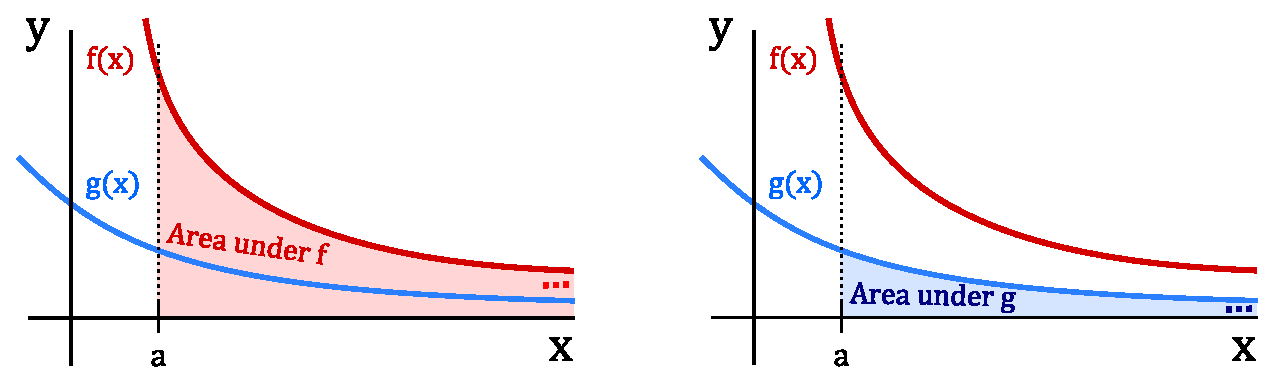
\includegraphics[width=6in]{images2/improper-integral-theory-3}$$

\begin{example}{Comparison Test}{Comparison Test}
Show that $\ds\int_2^\infty \frac{\cos^2x}{x^2} \,dx$ converges.
\end{example} 

\begin{solution}
We use the comparison test to show that it converges. 
Note that $0\leq \cos^2x\leq 1$ and hence 
$$0 \leq\frac{\cos^2x}{x^2}\leq\frac{1}{x^2}.$$
Thus, taking $f(x)=1/x^2$ and $g(x)=\cos^2x / x^2$ we have $f(x)\geq g(x)\geq 0$. 
One can easily see that $\ds\int_2^\infty \frac{1}{x^2}\,dx$ converges. 
Therefore, $\ds\int_2^\infty \frac{\cos^2x}{x^2} \,dx$ also converges.
\end{solution}


%%%%%%%%%%%%%%%%%%%%%%%%%%%%%%%%%%%%%%%%%%%%%%%%%
\Opensolutionfile{solutions}[ex]
\section*{Exercises for Section \ref{sec:ImproperIntegrals}}

\begin{enumialphparenastyle}

\begin{ex}
	Determine whether $\ds\int_1^{\infty}\frac{1}{x^2}\,dx$ is convergent or divergent.
	\begin{sol}
		Converges to 1.
	\end{sol}
\end{ex}

\begin{ex}
	Determine whether $\ds\int_e^{\infty}\frac{1}{x\sqrt{\ln x}}\,dx$ is convergent or divergent.
	\begin{sol}
		Diverges.
	\end{sol}
\end{ex}

\begin{ex}
	Evaluate the improper integral $\ds\int_0^{\infty}e^{-3x}\,dx$.
	\begin{sol}
		1/3
	\end{sol}
\end{ex}

\begin{ex}
	Determine if $\ds\int_1^e\frac{1}{x(\ln x)^2}\,dx$ is convergent or divergent. Evaluate it if it is convergent.
	\begin{sol}
		Divergent.
	\end{sol}
\end{ex}

\begin{ex}
	Show that $\ds\int_0^{\infty}e^{-x}\sin^2\left(\frac{\pi x}{2}\right)\,dx$ converges.
\end{ex}

\begin{ex}
	Evaluate $\ds\int_{-\infty}^{\infty}\frac{1}{x^2+1}\,dx$ and $\ds\int_{-\infty}^{\infty}\frac{x}{x^2+1}\,dx$.
\end{ex}

\begin{ex}
	Determine whether the following improper integrals are convergent or divergent. Evaluate those that are convergent.
	\begin{enumerate}
		\item	$\int_{0}^{\infty}\dfrac{1}{x^2+1}\,dx$
		\item	$\int_{0}^{\infty}\dfrac{x}{x^2+1}\,dx$
		\item	$\int_{0}^{\infty}e^{-x}(\cos x+\sin x)\,dx$. [Hint: What is the derivative of $-e^{-x}\cos x?$]
		\item	$\int_{0}^{\pi/2}\sec^{2}x\,dx$
		\item	$\int_{0}^{4}\dfrac{1}{(4-x)^{2/5}}\,dx$
	\end{enumerate}
	\begin{sol}
		\begin{enumerate}
			\item	$\pi/2$
			\item	divergent (to $\infty$)
			\item	1
			\item	divergent (to $\infty$)
			\item	$\frac{5}{3}(4^{3/5})$
		\end{enumerate}
	\end{sol}
\end{ex}

\begin{ex}
	Prove that the integral $\int_{1}^{\infty}\dfrac{1}{x^p}\,dx$ is convergent if $p>1$ and divergent if $0<p\leq 1$.
\end{ex}

\begin{ex}
	Suppose that $p>0$. Find all values of $p$ for which $\int_{0}^{1}\dfrac{1}{x^p}\,dx$ converges.
	\begin{sol}
		$0<p<1$
	\end{sol}
\end{ex}

\begin{ex}
	Show that $\int_{1}^{\infty}\dfrac{\sin^2 x}{x(\sqrt{x}+1)}\,dx$ converges.
\end{ex}

\end{enumialphparenastyle}